\chapter{Przygotowanie środowiska - automatyzacja}

Rozpoznanie numeru autobusu, ze względu na niewielką moc obliczeniową
urządzeń mobilnych, wymaga zastosowania segmentacji obrazu 
(najlepiej kilkustopniowej), czyli preselekcji obszarów potencjalnie
interesujących: fronty autobusów w~scenie, numery autobusów
we frontach itd. Poszczególne podprocesy powinny być
uszeregowane w~ten sposób, aby dane wejściowe - klatki obrazu - 
w~pierwszej kolejności były przetwarzane przez algorytmy o~najmniejszej
złożoności obliczeniowej. Dzięki temu
bardziej złożone i~intensywne obliczeniowo algorytmy będą operowały 
na mniejszych zbiorach danych, przez co czas przetwarzania ulegnie
skróceniu, a~otrzymane wyniki będą bardziej adekwatne.

Przykładowa sekwencja mogłaby wyglądać
w~sposób następujący:

\begin{enumerate}
    \item Przeszukiwanie klatki pod kątem wystąpienia frontu autobusu -
        wstępna segmentacja.
    \item Identyfikacja marki i~modelu (opcjonalne).
    \item Przeszukiwanie fragmentu reprezentującego front autobusu
        pod kątem numeru linii.
    \item Odczyt numeru z~odnalezionego fragmentu obrazu.
\end{enumerate}

Postępująca segmentacja obrazu powinna umożliwić rozpoznanie
numeru autobusu w~czasie rzeczywistym, niezależnie od klasy urządzenia.

Biorąc pod uwagę powyższe wymagania
w~ramach niniejszej pracy dyplomowej powinien powstać algorytm 
składający się co najmniej z~trzech niezależnych elementów. 
Każdy ze wspomnianych procesów musi zostać odpowiednio skonfigurowany
i~dostosowany do tego konkretnego zadania. Jedną z~najważniejszych, 
a~zarazem najtrudniejszych rzeczy jest osiągnięcie kompromisu 
między skutecznością, a wydajnością, do czego niezbędne są 
zautomatyzowane testy.

Do wstępnej segmentacji - lokalizacji frontu autobusu - najodpowiedniejszym
wydaje się być kaskadowy detektor dostępny w~bibliotece OpenCV. 
Wybór ten niesie za sobą konieczność przeprowadzeniu procesu uczenia
detektorów. Jest to bardzo czasochłonne przedsięwzięcie, 
wymaga dużych zbiorów danych uczących, zbioru testowego, a~wykonanie
jednego przebiegu programu może trwać nawet do kilkunastu godzin. 
W~następnych podrozdziałach 
przedstawione zostały narzędzia, których
zadaniem miała być maksymalna automatyzacja i~optymalizacja procesu uczenia
oraz weryfikacji zarówno skuteczności jak i~wydajności uzyskanych wersji
detektorów. W~dalszych podrozdziałach opisano kolejne
kroki algorytmu, a~także narzędzia służące w~ich przygotowaniu oraz 
weryfikacji.

Celem tego rozdziału było więc udokumentowanie prób przeprowadzonych
na drodze do osiągnięcia jak najbardziej zoptymalizowanego 
i~zautomatyzowanego procesu przygotowywania oraz testowania detektorów,
oraz innych elementów docelowego systemu.

\section{Wspomaganie pobierania filmów z serwisu YouTube}

Prace nad automatyzacją procesów rozpoczęto z~wielkim rozmachem.
Chęć poznawania nowych technologii, narzędzi i bibliotek
przyćmiła nieco zdrowy rozsądek. Jako pierwsza powstała wtyczka
do programu Firefox ułatwiającej pobieranie i wstępne katalogowanie filmów
udostępnianych za pośrednictwem serwisu YouTube.
Założenia oraz oczekiwania funkcjonalne wobec omawianego narzędzia były 
następujące:

\begin{enumerate}
    \item Wizualizacja stanu w~jakim znajduje się oglądany film - 
        możliwe są dwa stany:
    \begin{itemize}
        \item co najmniej jedna wersja filmu została już pobrana,
        \item film nie został pobrany w~żadnej wersji.
    \end{itemize}
    \item Możliwość pobrania wybranej wersji filmu w~odległości maksymalnie
        dwóch kliknięć licząc od poziomu przeglądania filmów w~serwisie,
    \item Tworzenie pliku CSV (\textit{ang. Comma Separated Value})
        z~danymi pobranych filmów, celem identyfikacji już pobranych
        pozycji. Plik powinien być tak skonstruowany aby można go było
        również wykorzystać do odtworzenia bazy filmów na dysku. W~razie
        awarii lub chęci przeprowadzenia całego procesu uczenia od
        początku.
\end{enumerate}

Powstały dwie wersje wtyczki. Pierwsza wkomponowana w~stronę portalu
jak na rysunku \ref{fig:firefoxplugin1}, oraz druga, 
ze względu na problemy 
z~interakcją z~interfejsem serwisu, umieszczona w~GUI samej przeglądarki.

\begin{figure}[h!]
    \caption{Przycisk rozwijanego menu, oraz wskaźnik stanu}
    \centering
    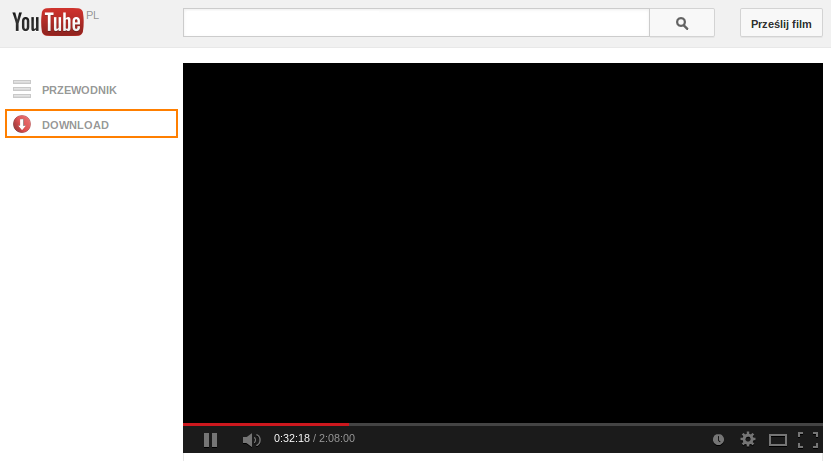
\includegraphics[width=0.9\textwidth]{img/env_yt_dwn_indicator}
    \label{fig:firefoxplugin1}
\end{figure}

Funkcjonalność drugiej wersji programu została drastycznie zmniejszona.
Ograniczała się do możliwości oznaczania wybranego filmu 
wraz z~jego wersją, oraz
eksportu tak utworzonych wpisów do pliku.
Przepływ sterowania dla drugiej wersji programu został przedstawiony
na diagramie \ref{fig:firefoxpluginflow}.

\begin{figure}[h!]
    \caption{Algorytm aktualizacji stanu wtyczki w wersji drugiej}
    \centering
    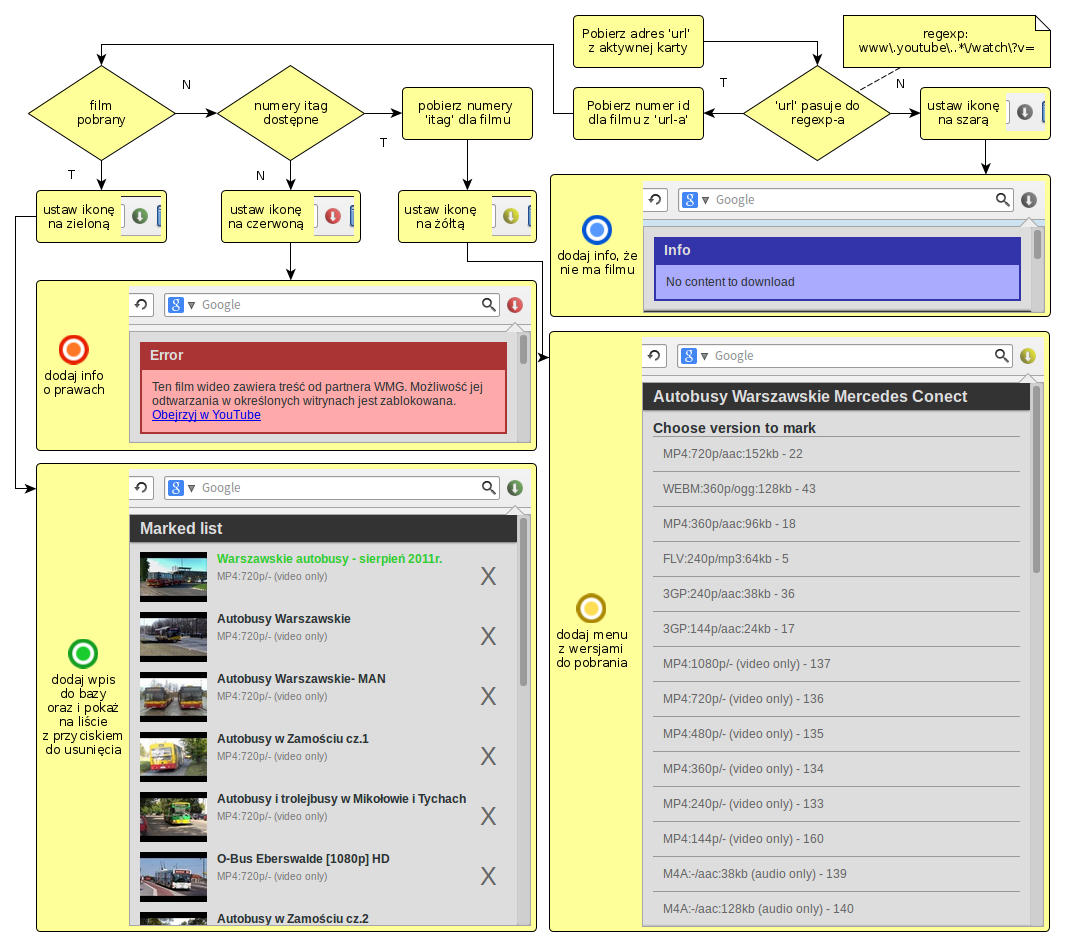
\includegraphics[width=0.9\textwidth]{img/env_yt_marker}
    \label{fig:firefoxpluginflow}
\end{figure}

Niestety pierwszy program ,,pomocniczy'' okazał się narzędziem nie
adekwatnym
(zbyt skomplikowanym i~pracochłonnym) do postawionego mu zadania. 
Okazało się, że
filmów zawierających fronty autobusów jest znacznie mniej niż mogło 
by się wydawać. Po znalezieniu 14 pozycji zawartość serwisu 
(w~kontekście frontów autobusów) nagle się
wyczerpała. Ostatecznie wielotygodniowe (dokładnie dwu) prace nad 
wtyczką do programu 
Firefox zaowocowały bazą czternastu pozycji w~formie pliku CSV,
co oczywiście o~wiele szybciej, prościej, wydajniej, taniej i~krótko 
mówiąc lepiej można
było wykonać bez implementowania żadnych narzędzi. 
Jedyne co pozostało to zdobyta wiedza
na temat: javascript, css, html, firefox: xul, addon-sdk, cfx. 

Kolejne narzędzia ,,pomocnicze'' implementowane były z~większą 
ostrożnością i~po
dłuższym przeanalizowaniu zagadnienia poddawanego automatyzacji.

\section{Tworzenie zbioru wejściowego do narzędzia train\_cascade}

Mając plik z~identyfikatorami filmów na serwisie YouTube wszystkie duże objętościowo
dane potrzebne przy tworzeniu wsadu od narzędzia uczącego można było zostawić
w~ich pierwotnym położeniu. Tworząc narzędzie wspomagające oznaczanie frontów
wzbogacono je o~możliwość odtworzenia osiągniętego stanu w~oparciu o~pliki konfiguracyjne.
Dodana funkcjonalność i~systematyczne archiwizowanie danych do zewnętrznego repozytorium
umożliwiły niezakłóconą kontynuację prac po awarii i~utracie lokalnej kopii.

Interfejsem narzędzia odpowiedzialnego za przygotowanie danych uczących był skrypt
napisany w~języku python:

\lstinputlisting{data/autocascader.txt}

Skrypt podobnie jak uprzednio opisana wtyczka był napisany 
nieco zbyt wcześnie. W~tym przypadku jednak nakład pracy jaki 
można było zautomatyzować był znacznie większy. Oznaczonych zostało 
bowiem kilka tysięcy klatek reprezentujących fronty autobusów
(w tym kilkaset frontów autobusów Solaris Urbino), oraz kilka tysięcy
obrazów tła. 

Po wyeksportowaniu plików roboczych na serwery serwisu GitHub
nadarzyła się okazja do przetestowania omawianego skryptu.
Podczas przenoszenia danych - wyłuskanych 
zdjęć z~podziałem na fronty, solarisy i~tła, nastąpiła awaria dysku
twardego. Posiadając jedynie pliki wskazujące klatki oraz plik 
z~danymi filmów udało się odtworzyć wszystkie wyłuskane i~oznaczone
zdjęcia. Po drobnych poprawkach w~skrypcie zaoszczędzono kilka wieczorów
poświęconych na przeglądanie i~wybieranie zdjęć.

\section{Automatyzacja procesu uczenia i~weryfikacji skuteczności
    detektorów kaskadowych - problemy pierwszej iteracji}

W~miarę jak prace nad algorytmem i~implementacją postępowały, powstawały
coraz to nowe narzędzia pomocnicze, których mnogość i~prostota nie
pozwalały na zamieszczenie ich szczegółowego opisu. 

Problem którego nie udało się zautomatyzować 
w~ramach pierwszej iteracji to weryfikacja skuteczności
całego algorytmu oraz poszczególnych jego elementów. Pierwszą
próbą weryfikacji skuteczności było prymitywne porównywanie współrzędnych
wykrytego fragmentu z~tak zwaną \textit{,,ground truth''} - oznaczonymi
wystąpieniami szukanych obiektów, wykonanymi na potrzeby uczenia 
detektorów. 
Przyjęty margines błędu - (+/-) 1/4 wysokości i~szerokości - skutkował dość
wysokimi uzyskanymi współczynnikami skuteczności. Podejście to okazało
się jednak zupełnie nieadekwatne do postawionego zadania.

\begin{figure}[h!]
    \caption{Błędne założenia przy implementacji narzędzi do
    weryfikacji skuteczności}
    \centering
    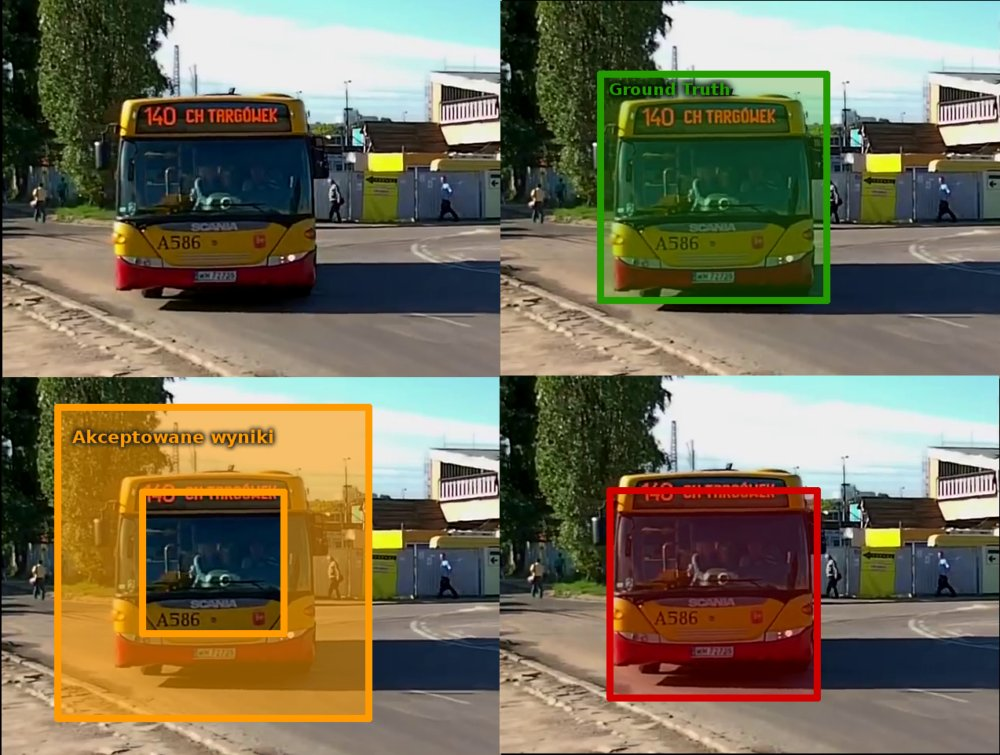
\includegraphics[width=0.9\textwidth]{img/env_benchmark_fail_1}
    \label{fig:autoverificationfail}
\end{figure}

Stosując przedstawianą metodę otrzymywano 
duży odsetek mocno nieprecyzyjnych oznaczeń
zaliczonych jako pozytywne. Niestety
z~punktu widzenia postawionego problemu -
odczytania numeru nadjeżdżającego autobusu - 
było to niedopuszczalne. Na rysunku 
\ref{fig:autoverificationfail} przedstawiono przykład - 
zaznaczony na czerwono - wykrycia zaliczonego
jako pozytywne, które uniemożliwia odczytanie numeru z~powodu obcięcia
jego górnej części.

Dodatkowym utrudnieniem była ostateczna forma zbioru wykorzystanego 
do uczenia detektorów. Pierwsze podejście do problemu nauki 
detektorów wykorzystywało pełne klatki zawierające interesujący obiekt
oraz plik tekstowy wskazujący współrzędne czworokąta okalającego.
Ogólny odsetek wykryć na takim zbiorze był zadowalający. 
Ostatecznie zrezygnowano z~przechowywania pełnych klatek na rzecz
wycinków reprezentujących wyłącznie instancje szukanych obiektów.
Było to spowodowane ograniczeniem przestrzeni dyskowej. Zbiór pełnych
klatek zajmował 32 GB, kiedy te same dane - fronty autobusów - po
przycięciu zajmowały nieco ponad 2 GB.

Niestety taka forma przechowywania danych 
- przycięte obrazy, reprezentujące fronty autobusów - spowodowała zafałszowanie 
wyników procesu automatycznej weryfikacji skuteczności.
Weryfikator uruchomiony na przyciętych obrazach wykazał
drastyczny spadek skuteczności tych samych detektorów w~stosunku
do wyników uzyskanych na poprzednim zbiorze testowym (pełne klatki
z~plikiem zawierającym współrzędne).
Rzetelna weryfikacja skuteczności była możliwa jedynie po ponownym przygotowaniu
zbioru testowego co było główną przyczyną 
całkowitego zaniechania automatycznych testów skuteczności
w~ramach pierwszej iteracji.


Za główny cel, postawiono jak najszybsze uruchomienie
aplikacji na urządzeniu. Mając działający prototyp, czyli
pewność, że aplikacja da się uruchomić, działa w~czasie zbliżonym
do rzeczywistego i~zwraca wyniki wskazujące na możliwość
osiągnięcia zadowalającej skuteczności można było spokojnie 
powrócić do weryfikacji i~późniejszego poprawiania
poszczególnych elementów systemu.

\section{Automatyczna weryfikacja detektorów - podejście drugie}

Pierwotny problem związany z~brakiem wystarczająco dużej liczby
obrazów reprezentujących fronty autobusów różnych typów został
rozwiązany dzięki zasobom udostępnianym za pośrednictwem serwisu
internetowego: \verb|http://www.phototrans.eu|.

Z~wykorzystaniem prostego skryptu napisanego w~języku Python pobrany
został próbny zbiór zdjęć reprezentujących pojazdy komunikacji
zbiorowej. Organizacja serwisu umożliwiła zastosowanie
podziału zbioru ze względu na numer linii, niestety
w~skład każdego zbioru wchodziły zarówno autobusy miejskie, dalekobieżne
jaki i~tramwaje. Ostatecznie pobrano 528 zestawów zdjęć reprezentujących
poszczególne linie, oraz zawierających średnio 40 zdjęć każdy, co
w~sumie dało 19367 obrazów, które trzeba było poddać weryfikacji.

W~celu weryfikacji detektorów frontów autobusów wybranych zostało 2000
zdjęć zawierających przody autobusów posiadających:

\begin{itemize}
    \item wyświetlacz diodowy z~numerem i~nazwą kierunku,
    \item numer linii w~lewym górnym rogu frontu.
\end{itemize}.

Ograniczenia wynikały ze względu na tendencje do wykrywania 
tego typu frontów przez przygotowane detektory, oraz
potrzebę uproszczenia przy wyszukiwaniu numeru linii w~znalezionym
froncie autobusu. Jednocześnie
był to zbiór na tyle obszerny, że tak przygotowany prototyp aplikacji byłby
w~pełni funkcjonalny w~wielu miastach (na przykład w~Warszawie - gdzie
wszystkie aktualnie wykorzystywane autobusy spełniają oba powyższe
ograniczenia).

Kolejnym narzędziem był skrypt przygotowujący zestaw wybranych 2000 zdjęć,
tak aby można było je wykorzystać w~procesie zarówno weryfikacji jak 
i~optymalizacji detektorów. Uruchomienie skryptu polegało na wyświetleniu
każdego ze zdjęć z~możliwością oznaczenia czworokąta okalającego front
(wykorzystano w~tym celu bibliotekę OpenCV). Dodatkowym ograniczeniem
było maksymalnie jedno wystąpienie frontu w~danym obrazie, co 
pozwalało na późniejsze wykorzystanie zbioru w~procesie
poszukiwania optymalnego współczynnika skalującego. Tak wprowadzone
dane umieszczane były w~nazwie każdego z~plików w~formie:
\verb|staranazwa-x_y_szerokosc_wysokosc.jpg|.

Proces weryfikacji przebiegał podobnie jak poprzednio. Rejestrowane były
poprawne oraz niepoprawne wykrycia, a~także ich brak. Ze względu na
większą dokładność pierwszego prototypowego detektora, margines
błędu zmniejszono z~1/4 wysokości i~szerokości na ich 1/5.
W~następnym rozdziale podjęto próbę systematyzacji otrzymanych wyników.
